\section*{Background}
In this section we explain some concepts we had to understand implementing our project. 
% Some "prerequisite" knowledge we assume is known: Socket Programming Protocols (TCP etc.), Interprocess Communication 
% Fussnote: HTTP Protocol Doc, CGI doc  

\subsection*{HTTP Protocol}
% historical (0.9 to 1.1). 
% Request types   
% structure (headers, message etc)
% headers (keep-alive)

\subsection*{Common Gateway Interface}
% why does it need cgi ? -> POST requests, backend services
% picture: 
% common gateway interface
% different types of implementation: fastCGI is the standard today 
The Common Gateway Interface (CGI) is a technology we encountered during our research on handling HTTP POST requests. CGI is an interface that defines how the web server interacts with external content-generating programs. This enables the creation of dynamic content, such as generating user-specific webpages or processing form submissions, and facilitates communication between the web server and the application backend service.

\begin{figure}[h]
	\centering
	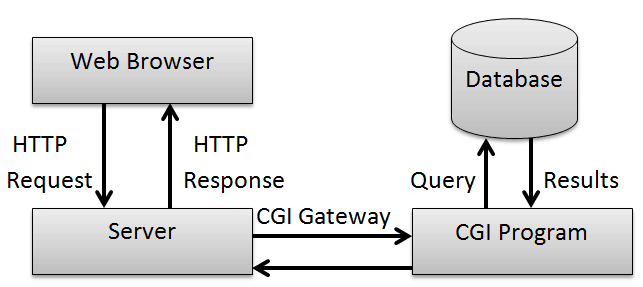
\includegraphics[width=\textwidth]{figures/Common-Gateway-Interface.png}
	\caption{The Common Gateway Interface}
\end{figure}

Here's how it works: When a request with a URL denoting a CGI script, like example.com/backend.cgi, enters the web server, the server locates the executable file called backend.cgi. It then spawns a process to execute the CGI script and communicates with this process via piped standard input/output and environment variables. After the CGI script sends its response to the web server, the server may verify the response and forward it to the client.\\

Although CGI is now quite outdated and less frequently used due to the inefficiency of spawning a new process for each request, enhanced versions such as FastCGI or SCGI are widely used. These versions improve performance by spawning CGI scripts only once. In our project we implemented the original CGI specification from 1997.

